%!TEX root = ../main.tex
\chapter{Richiami di trigonometria}

\section*{Funzioni trigonometriche}

Dato il triangolo rettangolo mostrato in figura di cateti $\displaystyle a$ e $\displaystyle b$, ipotenusa $\displaystyle c$ ed angolo $\displaystyle \vartheta $ opposto al cateto $\displaystyle a$, si definiscono:

\begin{equation*}
	\begin{array}{ l l }
		\sin \vartheta =\frac{a}{c} & \cos \vartheta =\frac{b}{c}\\
		[4mm]
		\tan \vartheta =\frac{a}{b} =\frac{\sin \vartheta }{\cos \vartheta } \ \ \ \  & \cot \vartheta =\frac{b}{a} =\frac{\cos \vartheta }{\sin \vartheta }
	\end{array}
\end{equation*}

\begin{figure}[htpb]
	\centering
	\tikzset{every picture/.style={line width=0.75pt}} %set default line width to 0.75pt

	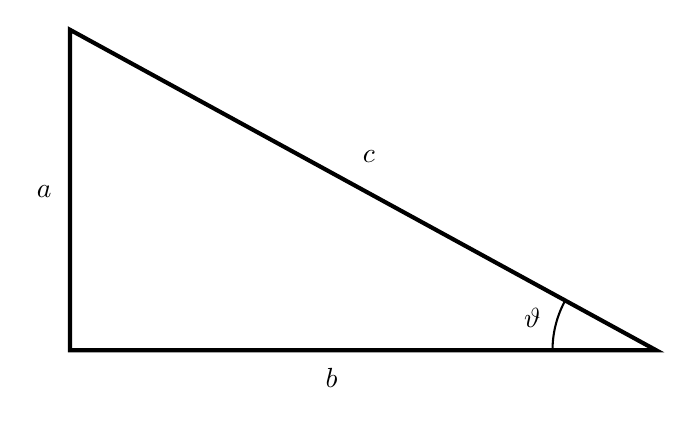
\begin{tikzpicture}[x=0.75pt,y=0.75pt,yscale=-1,xscale=1]
	%uncomment if require: \path (0,300); %set diagram left start at 0, and has height of 300

	%Shape: Right Triangle [id:dp9340776108358415]
	\draw  [line width=1.5]  (162,57) -- (444.5,211.44) -- (162,211.44) -- cycle ;
	%Shape: Arc [id:dp8374391809216872]
	\draw  [draw opacity=0] (394.5,211.86) .. controls (394.5,211.72) and (394.5,211.58) .. (394.5,211.44) .. controls (394.5,202.5) and (396.84,194.12) .. (400.95,186.86) -- (444.5,211.44) -- cycle ; \draw   (394.5,211.86) .. controls (394.5,211.72) and (394.5,211.58) .. (394.5,211.44) .. controls (394.5,202.5) and (396.84,194.12) .. (400.95,186.86) ;

	% Text Node
	\draw (384.8,196) node    {$\vartheta $};
	% Text Node
	\draw (149.6,134.8) node    {$a$};
	% Text Node
	\draw (288,224.8) node    {$b$};
	% Text Node
	\draw (306,118) node    {$c$};

	\end{tikzpicture}
\end{figure}

\section*{Identità trigonometriche}

Risultano le seguenti relazioni

\begin{equation*}
	\begin{array}{ c c }
		\sin \vartheta =\cos\left(\frac{\pi }{2} -\vartheta \right) & \cos \vartheta =\sin\left(\frac{\pi }{2} -\vartheta \right)\\
		[4mm]
		\cot \vartheta =\tan\left(\frac{\pi }{2} -\vartheta \right) & \sin^2 \vartheta +\cos^2 \vartheta =1\\
		[4mm]
		\cos^2 \vartheta =\frac{1}{1+\tan^2 \vartheta } & \sin^2 \vartheta =\frac{1}{1+\cot^2 \vartheta }\\
		[4mm]
		\cos 2\vartheta =\cos^2 \vartheta -\sin^2 \vartheta  & \sin 2\vartheta =2\sin \vartheta \cos \vartheta \\
		[4mm]
		\cos^2\frac{\vartheta }{2} =\frac{1+\cos \vartheta }{2} & \sin^2\frac{\vartheta }{2} =\frac{1-\cos \vartheta }{2}\\
		[4mm]
		\tan 2\vartheta =\frac{2\tan \vartheta }{1-\tan^2 \vartheta } & \tan\frac{\vartheta }{2} =\sqrt{\frac{1-\cos \vartheta }{1+\cos \vartheta }}
	\end{array}
\end{equation*}

Inoltre valgono le seguenti regole di somma:

\begin{equation*}
	\begin{array}{ c }
		\sin( \alpha \pm \beta ) =\sin \alpha \cos \beta \pm \cos \alpha \sin \beta \\
		[4mm]
		\cos( \alpha \pm \beta ) =\cos \alpha \cos \beta \mp \sin \alpha \sin \beta \\
		[4mm]
		\tan( \alpha \pm \beta ) =\frac{\tan \alpha \pm \tan \beta }{1\mp \tan \alpha \tan \beta }\\
		[4mm]
		\sin \alpha \pm \sin \beta =2\sin\left[\frac{1}{2}( \alpha \pm \beta )\right]\cos\left[\frac{1}{2}( \alpha \mp \beta )\right]\\
		[4mm]
		\cos \alpha +\cos \beta =2\cos\left[\frac{1}{2}( \alpha +\beta )\right]\cos\left[\frac{1}{2}( \alpha -\beta )\right]\\
		[4mm]
		\cos \alpha -\cos \beta =2\sin\left[\frac{1}{2}( \alpha +\beta )\right]\sin\left[\frac{1}{2}( \alpha -\beta )\right]\\
		[4mm]
		\sin \alpha \cos \beta =\frac{1}{2}[\sin( \alpha +\beta ) +\sin( \alpha -\beta )]\\
		[4mm]
		\cos \alpha \cos \beta =\frac{1}{2}[\cos( \alpha +\beta ) +\cos( \alpha -\beta )]\\
		[4mm]
		\sin^2 \alpha -\sin^2 \beta =\sin( \alpha +\beta )\sin( \alpha -\beta )\\
		[4mm]
		\cos^2 \alpha -\cos^2 \beta =\sin( \alpha +\beta )\sin( \beta -\alpha )
	\end{array}
\end{equation*}

Nel campo complesso valgono le seguenti relazioni

\begin{equation*}
	\begin{array}{ c }
		\sin z=\frac{1}{2i}\left( e^{iz} -e^{-iz}\right)\\
		[4mm]
		\cos z=\frac{1}{2}\left( e^{iz} +e^{-iz}\right)
	\end{array}
\end{equation*}

dette formule di Eulero; inoltre

\begin{equation*}
	\begin{array}{ c }
		e^{iz} =\cos z+i\sin z\\
		[4mm]
		e^{x+iy} =e^x(\cos y+i\sin y)
	\end{array}
\end{equation*}

\section*{Formule notevoli per un triangolo}

Dato il triangolo mostrato in figura di lati $\displaystyle a$, $\displaystyle b$ e $\displaystyle c$ ed angoli $\displaystyle \alpha$, $\displaystyle \beta $ e $\displaystyle \gamma$, valgono le seguenti relazioni:

\begin{equation*}
	\begin{array}{ c }
		\alpha +\beta +\gamma =\pi \\
		[4mm]
		\frac{a}{\sin \alpha } =\frac{b}{\sin \beta } =\frac{c}{\sin \gamma }\\
		[4mm]
		a^2 =b^2 +c^2 -2bc\cos \alpha
	\end{array}
\end{equation*}

\begin{figure}[htpb]
	\centering
	\tikzset{every picture/.style={line width=0.75pt}} %set default line width to 0.75pt

	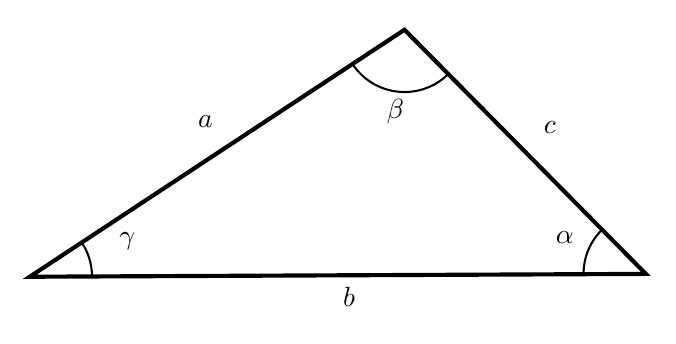
\begin{tikzpicture}[x=0.75pt,y=0.75pt,yscale=-1,xscale=1]
	%uncomment if require: \path (0,300); %set diagram left start at 0, and has height of 300

	%Shape: Boxed Polygon [id:dp5667907928913438]
	\draw  [line width=1.5]  (459.41,171.13) -- (162.59,172.5) -- (343.14,53.5) -- cycle ;
	%Shape: Arc [id:dp1523693032409319]
	\draw  [draw opacity=0] (187.57,155.88) .. controls (190.73,160.62) and (192.58,166.31) .. (192.59,172.43) -- (162.59,172.5) -- cycle ; \draw   (187.57,155.88) .. controls (190.73,160.62) and (192.58,166.31) .. (192.59,172.43) ;
	%Shape: Arc [id:dp8340291029684717]
	\draw  [draw opacity=0] (364.27,74.8) .. controls (358.85,80.18) and (351.38,83.5) .. (343.14,83.5) .. controls (332.66,83.5) and (323.44,78.13) .. (318.07,69.98) -- (343.14,53.5) -- cycle ; \draw   (364.27,74.8) .. controls (358.85,80.18) and (351.38,83.5) .. (343.14,83.5) .. controls (332.66,83.5) and (323.44,78.13) .. (318.07,69.98) ;
	%Shape: Arc [id:dp5702801543421352]
	\draw  [draw opacity=0] (429.41,171.18) .. controls (429.41,171.17) and (429.41,171.15) .. (429.41,171.13) .. controls (429.41,162.73) and (432.86,155.14) .. (438.42,149.7) -- (459.41,171.13) -- cycle ; \draw   (429.41,171.18) .. controls (429.41,171.17) and (429.41,171.15) .. (429.41,171.13) .. controls (429.41,162.73) and (432.86,155.14) .. (438.42,149.7) ;

	% Text Node
	\draw (209.6,155.2) node    {$\gamma $};
	% Text Node
	\draw (338.8,92.8) node    {$\beta $};
	% Text Node
	\draw (420.4,153.6) node    {$\alpha $};
	% Text Node
	\draw (247.2,97.6) node    {$a$};
	% Text Node
	\draw (413.2,100.8) node    {$c$};
	% Text Node
	\draw (316.4,182.4) node    {$b$};

	\end{tikzpicture}
\end{figure}